% !TeX root = ./rapport.tex
\chapter{Implémentation : front-end}

\paragraph{}Afin de représenter un circuit, nous avons défini les classes suivantes : \lstinline|BoardGrid| représente le \enquote{plateau} sur lequel est placé le circuit, \lstinline|Node| représente les nœuds de la grille du plateau, auxquels on peut connecter des éléments, \lstinline|Component| représente un composant du circuit (résistance, source de courant, etc.), \lstinline|Wire| représente un fil reliant deux nœuds. Enfin, la classe contenant la fonction \lstinline|main()| est \lstinline|MainWindow|. Il s'agit de la classe représentant la fenêtre et gérant les entrées claviers et les boutons. Son code est divisé en deux parties : une partie en XAML décrit la partie statique du code (division de l'interface, boutons), une autre en C\# gère les évènements et l'initialisation du circuit.

\paragraph{}Afin de gérer certaines interactions, trois autres classes sont nécessaires. Tout d'abord, déplacer un composant est facile, mais déplacer un fil, qui est composé de trois rectangles (il n'est pas forcément rectiligne), a nécessité l'ajout d'une classe \lstinline|WireDragger| qui gère le dragging d'un fil. Ensuite, pour éditer les propriétés d'un composant, telle la valeur d'une résistance par exemple, il est nécessaire de créer un pop-up avec les champs nécessaires. Cela ajoute la classe \lstinline|ComponentDialog|. Finalement, pour des raisons techniques qui seront expliquées plus bas, la sauvegarde du circuit nécessite l'ajout d'une classe \lstinline|SavedCircuit|.

\paragraph{}Cela donne en UML le diagramme de classes suivant (les accesseurs ne sont pas affichés pour simplifier le diagramme) :

\begin{figure}[H]
	\centering
	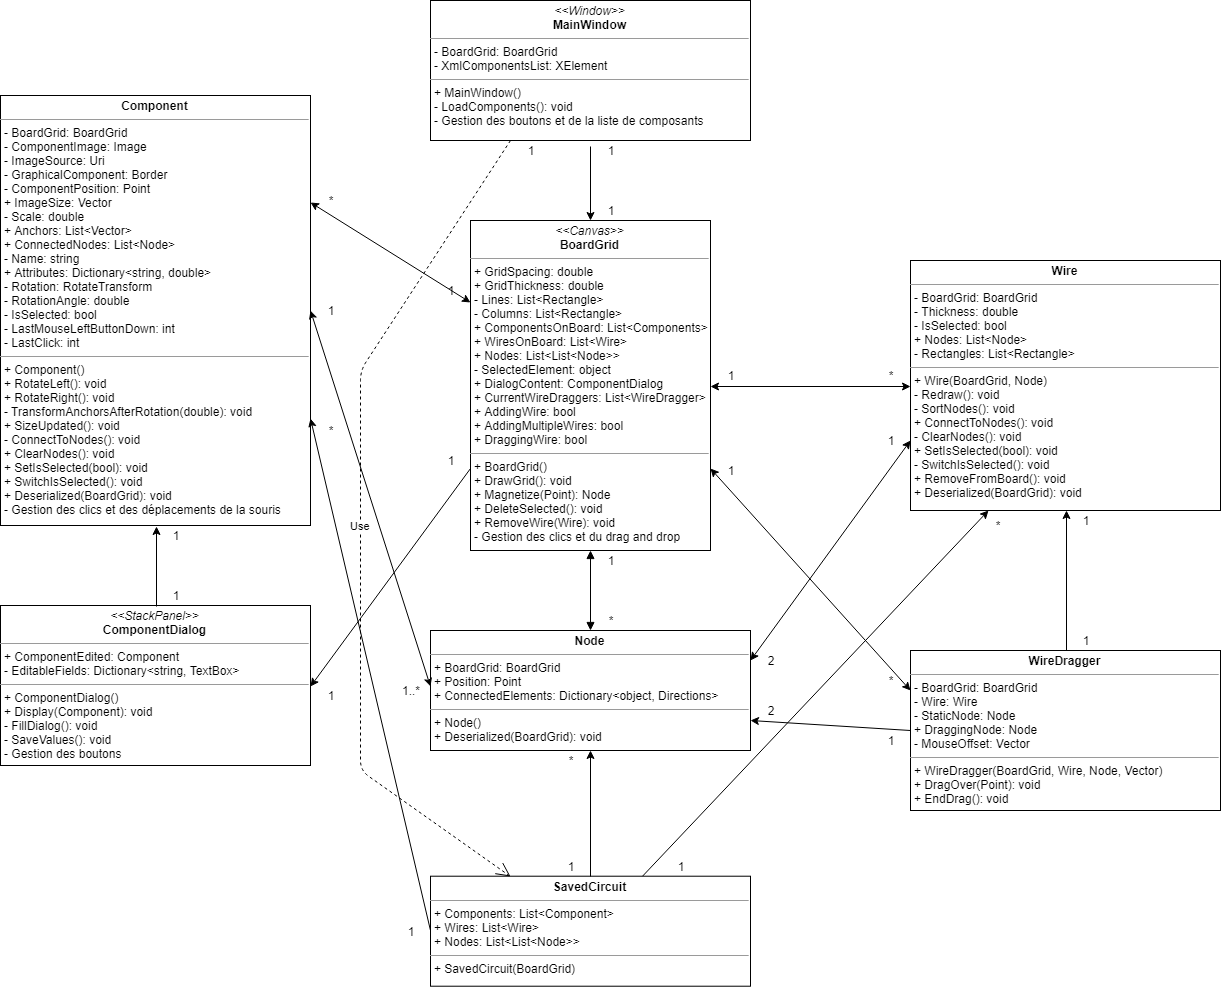
\includegraphics[width=0.7\textwidth]{diagrammeUML.png}
	\caption{Le diagramme de classes correspondant au front-end.}
	\label{fig:UML}
\end{figure}


\section{La classe \lstinline|MainWindow|}

\paragraph{}Cette classe la fenêtre et les éléments qui en dépendent directement. En XAML, certains éléments sont définis de manière statique : la barre d'outils et ses boutons d'édition : nouveau circuit, chargement, sauvegarde, rotation à gauche, rotation à droite, suppression, mode d'ajout de fil et mode d'ajout de multiples fils (celui-ci n'est visible que lorsque le mode précédent est actif ; le mode simple d'ajout de fil se termine après l'ajout du premier fil, celui-ci non). Ensuite, un panneau est défini sur la gauche de l'écran pour proposer les composants pouvant être ajoutés. Sur la droite, le reste de l'espace est réservé au circuit proprement dit : lors de l'initialisation, le programme lance une instance de BoardGrid et l'affiche dans cet espace.

\paragraph{}Cette classe contient aussi le code permettant de charger la liste des composants disponibles, qui est présente dans un fichier XML. Cela permet de modifier leurs caractéristiques rapidement et sans toucher au code source. Par exemple, la résistance est définie dans les lignes suivantes :

\lstinputlisting[language=xml, caption=Le XML définissant une source de tension alternative. Les ancres correspondent aux points de l'image sur lesquels un câble peut se brancher.]{Sources/source_tension_alternative.xml}


\section{La classe \lstinline|BoardGrid|}

\paragraph{}Cette classe représente le circuit dans son intégralité. Lors de son initialisation, elle dessine une grille constituée de rectangles horizontaux et verticaux et place des \lstinline|Node| aux intersections. Ensuite, elle gère l'ajout de composants et de fils, et en garde une liste. Une instance de \lstinline|BoardGrid| décrit donc parfaitement un circuit. 


\section{La classe \lstinline|Node|}

\paragraph{}La fonction \lstinline|Magnetize()| de \lstinline|BoardGrid| s'assure que tous les éléments (composants ou fils) sont bien ancrés sur un \lstinline|Node| du circuit : les positions possibles sont discrétisées. Un \lstinline|Node| conserve donc une liste de tous les éléments qui lui sont connectés. Lors de la simulation, un \lstinline|Node| correspond donc à un nœud du graphe représentant le circuit, et avoir une liste de toutes les instances de cette classe suffit à réaliser une simulation.


\section{Les classes \lstinline|Component| et \lstinline|ComponentDialog|}

\paragraph{}Un composant doit à la fois gérer les connections de ses ancres aux nœuds du circuit, pouvoir être déplacé, subir des rotations, être sélectionné, et pouvoir éditer ses attributs. \lstinline|Component| gère donc beaucoup d'événements, et gère tous les calculs pour que graphiquement, l'image représentant le composant soit toujours bien située et orientée. Lors d'un double-clic, une instance de \lstinline|ComponentDialog| est créée, qui permet de modifier les attributs du composant via un pop-up dont le contenu est généré dynamiquement en fonction du composant.


\section{Les classes \lstinline|Wire| et \lstinline|WireDragger|}

\paragraph{}Les fils sont des composants qui relient deux nœuds. Ils ne peuvent pas être déplacés individuellement, mais si un composant connecté à un film est déplacé, le fil le suivra. Afin de gérer ces déplacements, à chaque fois une instance de la classe \lstinline|WireDragger| est créée. Cette classe permet de gérer le déplacement du fil, lequel nécessite de définir est composé d'un bout fixe et d'un bout mobile qui suit la souris et se connecte à chaque mouvement au nœud le plus proche du pointeur.

\paragraph{}
